% -*- root: ../gvoysey-thesis.tex -*-
\chapter{Literature Review}
\label{chapter:literaturereview}
\thispagestyle{myheadings}
% set this to the location of the figures for this chapter. it may
% also want to be ../Figures/2_Body/ or something. make sure that
% it has a trailing directory separator (i.e., '/')!
\graphicspath{{2_LiteratureReview/Figures/}}
\section{Chapter Summary} % (fold)
\label{sec:review_summary}
This chapter lays out a review of the relevant literature this thesis relies on. First, an overview of the clinical significance and relevant neuroanatomy of cochlear synaptopathy are given.  Then, a review of the computational models that will be used is presented. 

% section review_summary (end)
\section{Cochlear Synaptopathy} % (fold)
\label{sec:cochlear_synaptopathy}
% section cochlear_synaptopathy (end)
Deafferentiation is the loss of one or more synapses between an Inner Hair Cell (IHC) and its innervating spiral ganglia. 

\cite{Kujawa2009Adding} showed in noise exposed mice that significant deafferentiation can occur with no permanent changes in threshold tuning curves and no hair cell death. \autoref{fig:furman-2} shows that deafferentiation was confirmed histologically by triple-staining cross--sections of the Organ of Corti post noise exposure.  This reveals a synaptic loss. 

\begin{figure}[htbp]
	\centering
	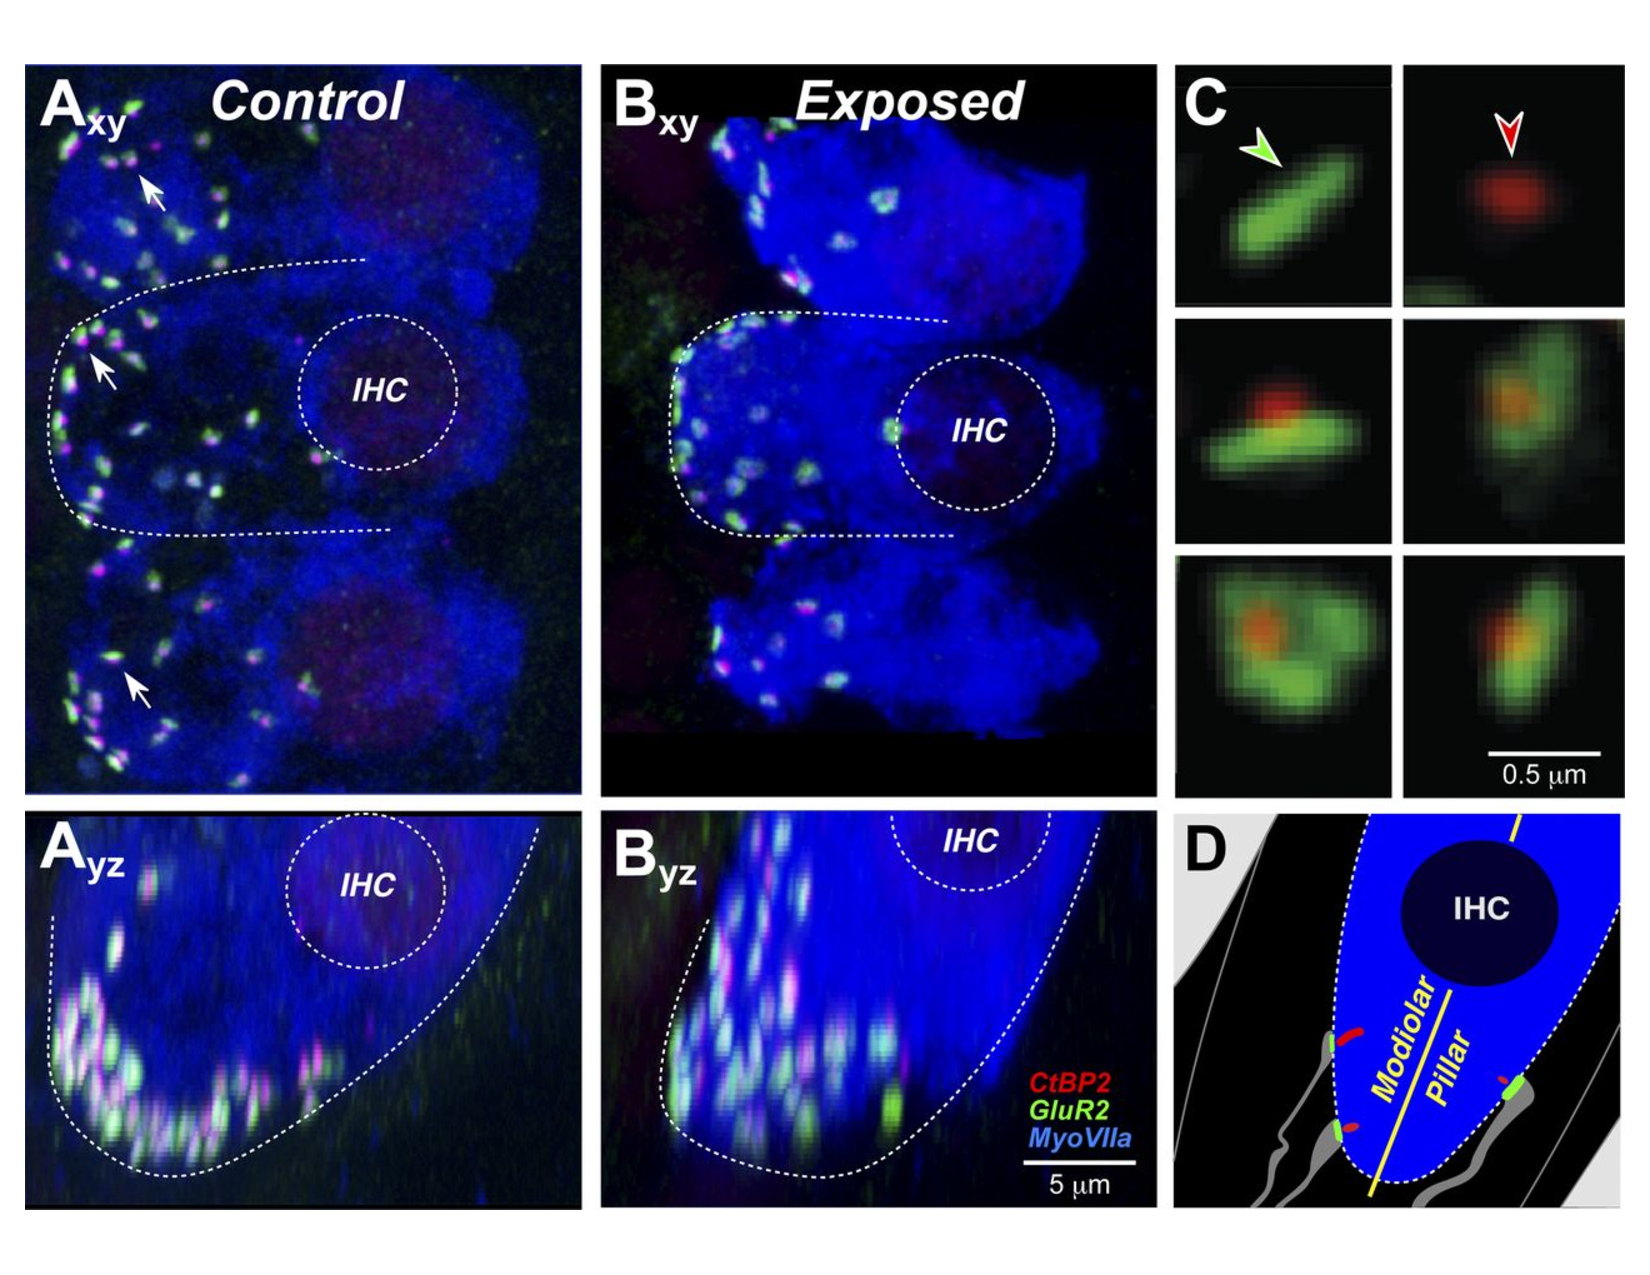
\includegraphics[width=0.95\textwidth]{furman-2.pdf}
	\caption[Deafferentation of Inner Hair Cells]{Deafferentiation of IHCs precedes hair cell death in noise exposed mice.  Figure is reprinted from \cite{Furman2013NoiseInduced}}
	\label{fig:furman-2}
\end{figure}


\cite{Sergeyenko2013AgeRelated} extended this work to demonstrate that this deafferentiation may also arise solely as a function of time.  In a study of mice aged 4 to 144 weeks that were never exposed to loud sounds, a similar loss of hair cell projections was observed.


\section{Physiology of the Auditory Nerve} % (fold)
\label{sec:physiology_of_the_auditory_nerve}
\subsection{Spontaneous Rates of Fibers} % (fold)
\label{sub:spontaneous_rates_of_fibers}
In the absence of stimulus, individual fibers of the auditory nerve exhibit a wide range of average firing rates: human AN fibers have spontaneous rates between 0--120 spikes/second.  Any individual fiber's spontaneous rate varies slowly over time, but will fall within a relatively narrow band.  The fibers of the auditory nerve are divided into two, or sometimes three, categories: low-, medium-, and high spontaneous rate (SR).  Different authors assign different maximum firing rates to each category:~\cite{Temchin2008Threshold} categorizes SRs below 18 spikes/second to be ``low/medium'', and anything above that to be ``high''.  Others, such as~\cite{Liberman1978AuditoryNerve}, define only two categories.  
% subsection spontaneous_rates_of_fibers (end)
\subsection{Low Spontaneous Rate Fibers Suffer Selective Losses} % (fold)
\label{sub:low_spontaneous_rate_fibers_suffer_selective_losses}
\cite{Furman2013NoiseInduced} and others have demonstrated that noise-induced cochlear synaptopathy is selective for low-SR fibers, particularly at high frequencies.

\begin{figure}[htbp]
	\centering
	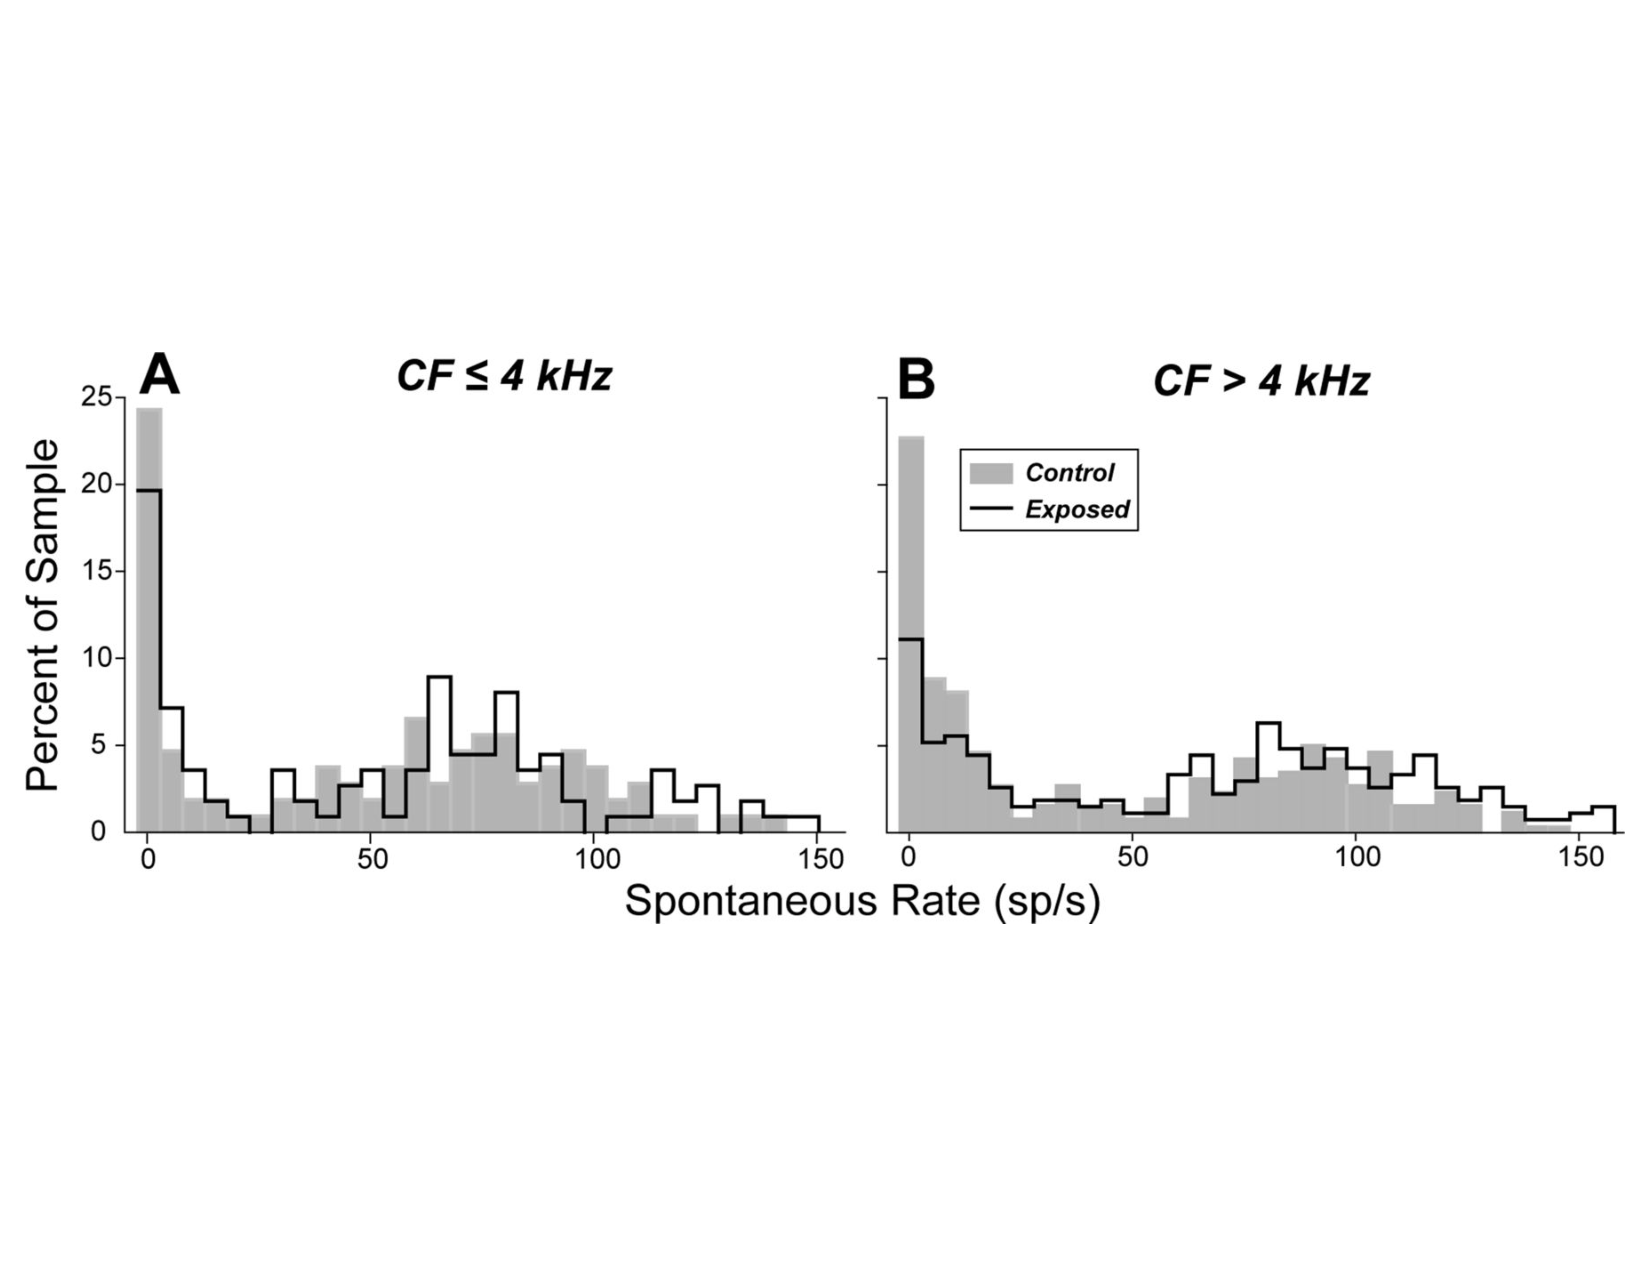
\includegraphics[width=0.95\textwidth]{furman-5.pdf}
	\caption[Synaptopathy is Selective]{Synaptopathy is selective for fibers with low spontaneous rates, and particularly selective for low-SR fibers at high frequencies. Figure reprinted from \cite{Furman2013NoiseInduced}}
	\label{fig:label}
\end{figure}

\section{Relevant Functional Neuroanatomy of the Auditory Midbrain} % (fold)
\label{sec:relevant_functional_neuroanatomy_of_the_auditory_midbrain}
\subsection{The Cochlear Nucleus} % (fold)
\label{sub:the_cochlear_nucleus}
The primary projection from the AN is the Cochlear Nucleus, the first auditory relay station located in the ipsilateral medulla of the brainstem.  
\subsection{The Dorsal Cochlear Nucleus} % (fold)
\label{sub:the_dorsal_cochlear_nucleus}
\cite{Ryugo2008Projections}
\subsubsection{The Small Cap Area} % (fold)
\label{ssub:the_small_cap_area}

% subsubsection the_small_cap_area (end)
% subsection the_dorsal_cochlear_nucleus (end)
\subsection{The Ventral Cochlear Nucleus} % (fold)
\label{sub:the_ventral_cochlear_nucleus}
While the VCN is critically important for the processing of binaural phenomena ()
% subsection the_ventral_cochlear_nucleus (end)
\subsection{The Inferior Colliculus} % (fold)
\label{sub:the_inferior_colliculus}
The IC has long been regarded as the last pre-thalamic obligate waystation for ascending auditory information. 
% subsection the_inferior_colliculus (end)
% section functional_neuroanatomy_of_the_auditory_midbrain (end)

\section{Auditory Modeling Environments} % (fold)
\label{sec:auditory_modeling_environments}
\subsection{The Carney Models} % (fold)
\label{sub:the_carney_models}
\subsubsection{The Zilany and Bruce Models} % (fold)
\label{ssub:zilany_and_bruce_2009_2014}

% subsubsection zilany_and_bruce_2009_2014 (end)
\subsubsection{Modulation Transfer Functions in the Inferior Colliculus} % (fold)
\label{ssub:modulation_transfer_functions_in_the_inferior_colliculus}

% subsubsection modulation_transfer_functions_in_the_inferior_colliculus (end)
% subsection the_carney_models (end)

\subsection{The Verhulst Model} % (fold)
\label{sub:the_verhulst_model}

% subsection the_verhulst_model (end)

% section auditory_modeling_environments (end)

\section{Objective Measures of Cochlear Synaptopathy} % (fold)
\label{sec:objective_measures_of_cochlear_synaptopathy}

% section objective_measures_of_cochlear_synaptopathy (end)
